\documentclass[tikz,border=10pt]{standalone}
\usepackage{amssymb}
\usetikzlibrary{arrows.meta, bending, decorations.markings, calc, shapes.geometric}

\tikzset{
  glueArrow/.style={-{Stealth[length=3mm]}, very thick, shorten >=2pt, shorten <=2pt},
  pathArrow/.style args={#1}{
    postaction={decorate},
    decoration={markings, mark=at position #1 with {\arrow[scale=1.5]{Stealth}}}
  },
  cycleLines/.style={very thick, draw=black},
  dotBase/.style={circle, inner sep=1.2pt},
  dotBlue/.style={dotBase, fill=blue},
  dotRed/.style={dotBase, fill=red},
  dotBlueBack/.style={dotBase, fill=blue!80, opacity=0.4},
  dotRedBack/.style={dotBase, fill=red!80, opacity=0.4}
}

\begin{document}
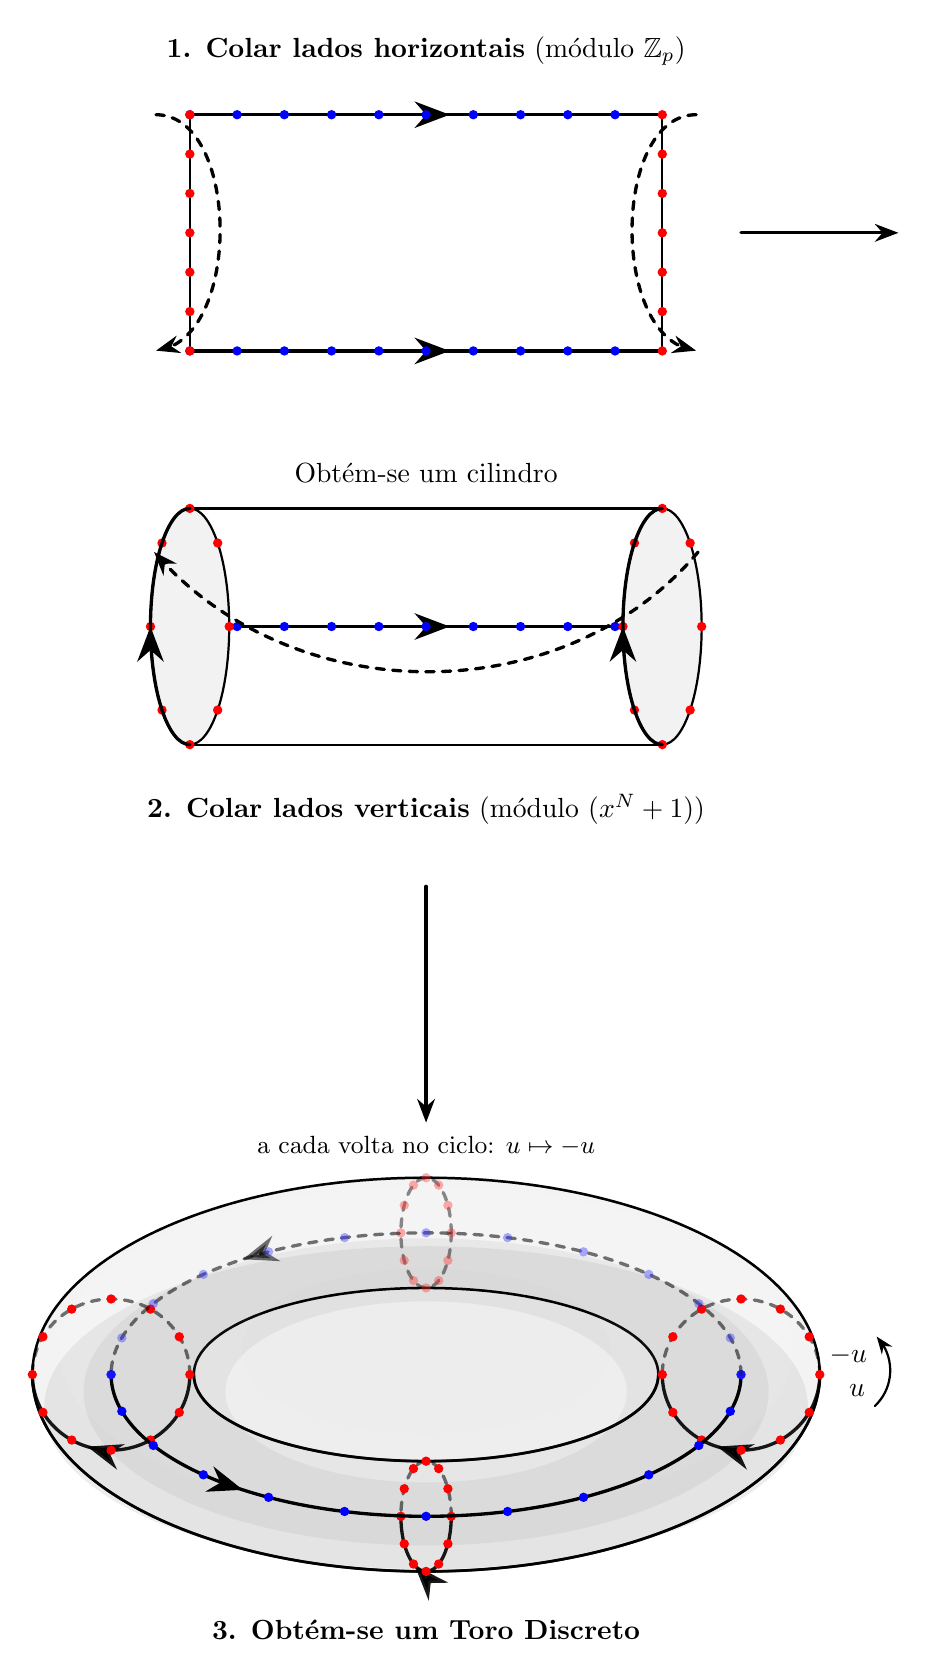
\begin{tikzpicture}[line cap=round, line join=round]

% ------------------------------------------------------------
% PARTE 1: O RETÂNGULO
% ------------------------------------------------------------
\begin{scope}[yshift=0cm]
  \coordinate (A) at (0, 0);
  \coordinate (B) at (6, 0);
  \coordinate (C) at (6, 3);
  \coordinate (D) at (0, 3);

  \draw[thick] (A) -- (B) -- (C) -- (D) -- cycle;

  \draw[cycleLines, pathArrow=0.55] (A) -- (B);
  \draw[cycleLines, pathArrow=0.55] (D) -- (C);

  \foreach \x in {0, 0.6, ..., 6} {
    \node[dotBlue] at (\x, 0) {};
    \node[dotBlue] at (\x, 3) {};
  }
  \foreach \y in {0, 0.5, ..., 3} {
    \node[dotRed] at (0, \y) {};
    \node[dotRed] at (6, \y) {};
  }

  \draw[glueArrow, dashed, bend left=90]  ($(D)+(-0.5,0)$) to ($(A)+(-0.5,0)$);
  \draw[glueArrow, dashed, bend right=90] ($(C)+(0.5,0)$)  to ($(B)+(0.5,0)$);

  \node[above] at (3, 3.5) {\textbf{1. Colar lados horizontais} (módulo $\mathbb{Z}_p$)};

  \draw[-{Stealth[length=3mm]}, very thick] (7, 1.5) -- (9, 1.5);
\end{scope}

% ------------------------------------------------------------
% PARTE 2: O CILINDRO
% ------------------------------------------------------------
\begin{scope}[yshift=-5cm]
  \draw[thick] (0, 3) -- (6, 3);
  \draw[thick] (0, 0) -- (6, 0);

  \draw[cycleLines, pathArrow=0.55] (0, 1.5) -- (6, 1.5);
  \foreach \x in {0, 0.6, ..., 6} {
    \node[dotBlue] at (\x, 1.5) {};
  }

  \draw[thick, fill=gray!10] (0, 1.5) ellipse (0.5 and 1.5);
  \foreach \ang in {0, 45, ..., 315} {
    \node[dotRed] at ({0 + 0.5*cos(\ang)}, {1.5 + 1.5*sin(\ang)}) {};
  }

  \draw[thick, fill=gray!10] (6, 1.5) ellipse (0.5 and 1.5);
  \foreach \ang in {0, 45, ..., 315} {
    \node[dotRed] at ({6 + 0.5*cos(\ang)}, {1.5 + 1.5*sin(\ang)}) {};
  }

  \draw[cycleLines, pathArrow=0.5] (0,0) arc[start angle=270, end angle=90, x radius=0.5, y radius=1.5];
  \draw[cycleLines, pathArrow=0.5] (6,0) arc[start angle=270, end angle=90, x radius=0.5, y radius=1.5];

  \draw[glueArrow, dashed, bend left=50] (6.5, 2.5) to (-0.5, 2.5);

  \node[above] at (3, 3.2) {Obtém-se um cilindro};
  \node[below] at (3, -0.5) {\textbf{2. Colar lados verticais} (módulo $(x^N + 1)$)};
\end{scope}

\draw[-{Stealth[length=3mm]}, very thick] (3, -6.8) -- (3, -9.8);

% ------------------------------------------------------------
% PARTE 3: O TORO (SEM \clip)
% ------------------------------------------------------------
\begin{scope}[yshift=-13cm, xshift=3cm]

  % --- Parâmetros do toro ---
  \def\RoutX{5}   \def\RoutY{2.5}
  \def\RinX{2.95} \def\RinY{1.10}

  % Órbita dos centros (ciclo maior)
  \def\MjRX{4} \def\MjRY{1.8}

  % ============================================================
  % TAMANHOS DOS CÍRCULOS MENORES (AJUSTE AQUI)
  % 0 e 180 (lados) -> LR
  % 90 e 270 (topo/baixo) -> TB
  % ============================================================
  \def\mrXLR{1.0} \def\mrYLR{0.96} % lados (0,180)
  \def\mrXTB{0.32} \def\mrYTB{0.70} % topo/baixo (90,270)

  % --- Sombra projetada ---
  \path[fill=black, opacity=0.07]
    (0,-0.42) ellipse[x radius=4.85cm, y radius=2.05cm];

  % --- Corpo do toro (anel base) ---
  \path[even odd rule, fill=gray!50, fill opacity=0.18, draw=black, line width=0.9pt]
    (0,0) ellipse[x radius=\RoutX cm, y radius=\RoutY cm]
    (0,0) ellipse[x radius=\RinX cm,  y radius=\RinY cm];

  % --- Sombra interna (anel deslocado) ---
  \path[even odd rule, fill=black, opacity=0.05]
    (0,-0.22) ellipse[x radius=4.35cm, y radius=1.95cm]
    (0,-0.22) ellipse[x radius=2.55cm, y radius=1.15cm];

  % --- Realce superior (anel deslocado) ---
  \path[even odd rule, fill=white, opacity=0.06]
    (0,0.30) ellipse[x radius=4.65cm, y radius=2.10cm]
    (0,0.30) ellipse[x radius=2.35cm, y radius=1.05cm];

  % --- Bordas (rims) ---
  \draw[black, opacity=0.30, dashed, line width=0.9pt]
    (-\RoutX,0) arc[start angle=180, end angle=0, x radius=\RoutX cm, y radius=\RoutY cm];
  \draw[black, opacity=0.85, line width=1.0pt]
    (\RoutX,0) arc[start angle=0, end angle=-180, x radius=\RoutX cm, y radius=\RoutY cm];

  \draw[black, opacity=0.28, dashed, line width=0.9pt]
    (-\RinX,0) arc[start angle=180, end angle=0, x radius=\RinX cm, y radius=\RinY cm];
  \draw[black, opacity=0.85, line width=1.0pt]
    (\RinX,0) arc[start angle=0, end angle=-180, x radius=\RinX cm, y radius=\RinY cm];

  % ============================================================
  % CÍRCULOS MENORES (4 apenas): 0, 90, 180, 270
  % Profundidade simples: tcY>0 = atrás (desenha primeiro)
  % ============================================================

  % --- atrás primeiro ---
  \foreach \torusAng in {0,90,180,270} {
    \pgfmathsetmacro{\tcX}{\MjRX*cos(\torusAng)}
    \pgfmathsetmacro{\tcY}{\MjRY*sin(\torusAng)}

    % Seleciona tamanho do círculo menor conforme o ângulo
    \def\mrx{\mrXTB}\def\mry{\mrYTB} % padrão: topo/baixo
    \ifnum\torusAng=0   \def\mrx{\mrXLR}\def\mry{\mrYLR}\fi
    \ifnum\torusAng=180 \def\mrx{\mrXLR}\def\mry{\mrYLR}\fi

    \ifdim \tcY pt > 0pt
      \begin{scope}[shift={(\tcX,\tcY)}]
        \draw[cycleLines, dashed, opacity=0.45]
          (\mrx,0) arc[start angle=0, end angle=-180, x radius=\mrx cm, y radius=\mry cm];
        \draw[cycleLines, dashed, opacity=0.45]
          (\mrx,0) arc[start angle=0, end angle=180, x radius=\mrx cm, y radius=\mry cm];

        \foreach \angSlice in {0,30,...,330} {
          \node[dotRedBack] at ({\mrx*cos(\angSlice)}, {\mry*sin(\angSlice)}) {};
        }
      \end{scope}
    \fi
  }

  % --- frente depois ---
  \foreach \torusAng in {0,90,180,270} {
    \pgfmathsetmacro{\tcX}{\MjRX*cos(\torusAng)}
    \pgfmathsetmacro{\tcY}{\MjRY*sin(\torusAng)}

    % Seleciona tamanho do círculo menor conforme o ângulo
    \def\mrx{\mrXTB}\def\mry{\mrYTB}
    \ifnum\torusAng=0   \def\mrx{\mrXLR}\def\mry{\mrYLR}\fi
    \ifnum\torusAng=180 \def\mrx{\mrXLR}\def\mry{\mrYLR}\fi

    \ifdim \tcY pt > 0pt
      % atrás: não desenha aqui
    \else
      \begin{scope}[shift={(\tcX,\tcY)}]
        \draw[cycleLines, pathArrow=0.6, opacity=0.90]
          (\mrx,0) arc[start angle=0, end angle=-180, x radius=\mrx cm, y radius=\mry cm];
        \draw[cycleLines, dashed, opacity=0.55]
          (\mrx,0) arc[start angle=0, end angle=180, x radius=\mrx cm, y radius=\mry cm];

        \foreach \angSlice in {0,30,...,330} {
          \node[dotRed] at ({\mrx*cos(\angSlice)}, {\mry*sin(\angSlice)}) {};
        }
      \end{scope}
    \fi
  }

  % ============================================================
  % CICLO MAIOR
  % ============================================================
  \draw[cycleLines, pathArrow=0.25]
    (-\MjRX,0) arc[start angle=180, end angle=360, x radius=\MjRX cm, y radius=\MjRY cm];
  \foreach \ang in {180,195,...,360} {
    \node[dotBlue] at ({\MjRX*cos(\ang)}, {\MjRY*sin(\ang)}) {};
  }

  \draw[cycleLines, dashed, opacity=0.55, pathArrow=0.75]
    (\MjRX,0) arc[start angle=0, end angle=180, x radius=\MjRX cm, y radius=\MjRY cm];
  \foreach \ang in {0,15,...,180} {
    \node[dotBlueBack] at ({\MjRX*cos(\ang)}, {\MjRY*sin(\ang)}) {};
  }

  % --- Anotação negacíclica no ciclo maior ---
  \node[above] at (0, {\MjRY + 0.85}) {\small a cada volta no ciclo: $u \mapsto -u$};

% ============================================================
  % NOVO: Rótulos e Seta u -> -u (no círculo a 0 graus)
  % ============================================================
  % Posicionamos próximo ao círculo da direita (MjRX, 0)
  % Usamos coordenadas relativas para acompanhar ajustes de tamanho
  \node (plusU)  [below right] at (\MjRX + 1.25, 0) {$u$};
  \node (minusU) [above right] at (\MjRX + 1, 0)  {$-u$};

\begin{scope}[shift={({\MjRX},0)}, xscale=-1, shift={({-\MjRX},0)}]
  \draw[-{Stealth[length=2.2mm]}, thick, black]
    (plusU.south east) to[bend left=45] (minusU.north east);
\end{scope}



  \node[below] at (0, -3) {\textbf{3. Obtém-se um Toro Discreto}};

\end{scope}

\end{tikzpicture}
\end{document}
